\documentclass[a4paper,12pt]{article}

\usepackage[utf8]{inputenc}
\usepackage[italian]{babel}
\usepackage{graphicx}
\usepackage{amsmath}
\usepackage{hyperref}
\usepackage{geometry}
\geometry{top=2.5cm, bottom=2.5cm, left=3cm, right=3cm}
\title{Progetto di Casa Domotica}
\author{Tagliapietra, Mega, Foresto - Itts Vito Volterra \\}
\date{\today}
\begin{document}
\maketitle
\begin{figure}[h!]
    \vspace{-0.8cm}
    \centering
    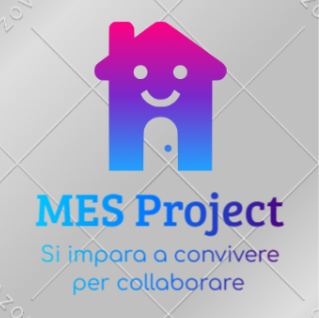
\includegraphics[width=0.3\textwidth]{logoProgetto.png} 
    \vspace{-0.5cm}
\end{figure}
\begin{abstract}
Questo documento è la documentazione del nostro progetto di Sistemi e Reti. Descrive il progetto di una casa domotica, che integra diverse tecnologie per migliorare il comfort, la sicurezza e l'efficienza energetica degli ambienti. Il sistema si basa su una rete di dispositivi intelligenti che possono essere controllati tramite un'applicazione centrale che gestiamo noi personalmente.
\end{abstract}
\begin{center}
    \begin{tabular}{|c|c|c|c|}
       \hline 
       Versione & Data & Autore & Docente \\
       \hline 
       1.2 & 28/03/2025 & MES Project & Tollot Lucilla \\
    \end{tabular}
\end{center}
\tableofcontents
\section{Introduzione}
Questo progetto è stato commissionato dal proprietario di una residenza per installare apparecchiature domotiche con lo scopo di migliorare la qualità della vita nell’abitazione. L’obiettivo principale è creare una rete domotica efficiente, evitando sprechi di risorse e ottimizzando i tempi di lavoro.
Il progetto prevede la produzione di documentazione, la realizzazione di un modello grafico e l’installazione del sistema domotico.
\section{Obiettivi del Progetto}
Il progetto si propone di:
\begin{itemize}
    \item Implementare un sistema di accensione e spegnimento da remoto per illuminazione,          
    climatizzazione e riscaldamento.
    \item Monitorare e gestire i consumi energetici attraverso dispositivi intelligenti.
    \item Integrare un sistema di controllo vocale per semplificare le operazioni quotidiane.
\end{itemize}

\section{Funzionalità.}
Queste sono le funzione del nostro progetto:
\begin{itemize}
    \item Domotizzazione della casa
    \item Scenari impostabili
    \item Gestione delle luci 
    \item Controllo tramite un'interfaccia web 
\end{itemize}

\section{Tecnologie Utilizzate}
Per realizzare il sistema domotico sono state utilizzate le seguenti tecnologie:
\begin{itemize}
    \item \textbf{Rasberry PI}: utilizzato come centro di controllo per gestire i dispositivi connessi.
    \item \textbf{Apparecchiature wireless}: conformi agli standard IEEE 802.11, come Wi-Fi e Zigbee.
    \item \textbf{Sensori di temperatura}: per monitorare e regolare l'ambiente domestico.
    \item \textbf{Sito web mobile}:  permette agli utenti di controllare i dispositivi da remoto.
    \item \textbf{Sistemi di intelligenza artificiale}: per ottimizzare i consumi energetici in base alle abitudini degli utenti.
\end{itemize}

\section{Progettazione del Sistema}
Il sistema domotico è composto da diversi componenti principali:
\begin{itemize}
    \item \textbf{Unità di Controllo Centrale}: una Raspberry Pi che funge da hub per comunicare con tutti i dispositivi.
    \item \textbf{Sensori e Attuatori}: dispositivi installati in casa che monitorano e controllano l'ambiente, come luci, serrature, sensori di temperatura e movimento.
    \item \textbf{Interfaccia Utente}: un'interfaccia web che consente di gestire il sistema da remoto.
    \item \textbf{Packet Tracer}: Tramite utilizzo del programma cisco packet tracer andiamo a progettare la futura rete.
\end{itemize}

\section{Realizzazione}
La realizzazione del progetto è avvenuta in diverse fasi:
\begin{enumerate}
    \item \textbf{Progettazione Hardware:}: scelta dei dispositivi da utilizzare, come i sensori di movimento, le luci intelligenti.
    \item \textbf{Installazione dei Dispositivi}: configurazione e collegamento dei vari dispositivi alla rete domestica.
    \item \textbf{Sviluppo Software}: creazione dell'app mobile e sviluppo dei programmi di controllo per il Raspberry Pi.
    \item \textbf{Test e Ottimizzazione}: verifica del corretto funzionamento del sistema e ottimizzazione delle performance.
\end{enumerate}

\section{Conclusioni}
L’obiettivo del progetto è completarlo nel minor tempo possibile, ottimizzando l’impiego delle risorse. I nostri tecnici eseguiranno test approfonditi sul sistema prima della consegna definitiva. Si auspica che l’integrazione dei sistemi domotici semplifichi la vita quotidiana dei residenti.

\section{Prospettive Future}
Il sistema è stato progettato che in futuro possa essere ampliato da chiunque così se in futuro escono tecnologie migliori si può pensare ad un aggiornamento delle apparecchiature installate precedentemente.


\end{document}
